\section{Automatic Scene Conversion} 
\label{sec:systemarch}

Our system consists of two main components: an {\it import module} that reads an arbitrary scene file format and generates an equivalent description in a {\it canonical} scene representation; and an {\it export module} that takes a canonical representation and exports it to a target rendering system file format. The complete process is illustrated in Figure \ref{fig:sysarch}. 
Currently, our system supports \textit{PBRT v-3}~\cite{PBRT:v3}, \textit{Mitsuba}~\cite{mitsuba}, and \textit{LuxRender}~\cite{luxrender}, as these are three of the most popular rendering systems.
This architecture, however, is quite flexible. Supporting additional rendering systems only requires specializing the import and export methods to handle the new formats. Moreover, it can be easily integrated with the API described in~\cite{Santos:2018:FBKSD}.   
%
Next, we describe the main components of our system.

%Our Proof of Concept (PoC) encompassed \textit{PBRT} \cite{pbrt}, \textit{Mitsuba}
%\cite{mitsuba} and \textit{LuxRender} \cite{luxrender}, as these are three of
%the most popularly used renderers in the community. This architecture, however,
%is easily extensible: adding other renderers would be a simple task of writing
%an import and a conversion module.



%converting pipeline is subdivided into three main states: the \textbf{Import
%Module}, the \textbf{Canonical Scene Representation} and the \textbf{Conversion
%Module}, as illustrated in Figure \ref{fig:sysarch}. Given an arbitrary input
%file format, our converter is able to import the scene and transform it into a
%generic, canonical representation and then export it to different output
%formats.

\begin{figure}[h]
\centering
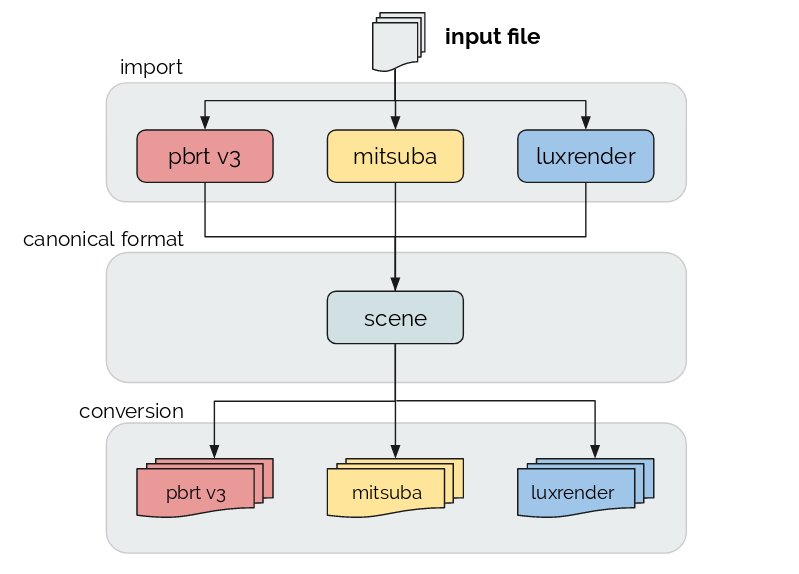
\includegraphics[width=0.8\linewidth]{figs/3_system_architecture/architecture.png}
\caption{Our scene conversion pipeline. An input scene description is converted to a canonical representation, which, in turn, can be exported to a target rendering system format.}
\label{fig:sysarch}
\end{figure}

\subsection{The Import Module}
Most physically-based renderers subdivide the scene description in two main sections:
%Usually, it is divided into two sections: 
{\it scene-wide rendering options} and {\it world block}. The former defines the rendering settings, while the latter describes the scene geometry and materials.
%
The import module parses the input scene files and translates each directive into a canonical
representation. Since rendering systems use proprietary file format, both the import and export modules have to be specialized for each renderer.

PBRT and LuxRender scene descriptions consist of structured text statements \red{(see XXX)}. We generated parsers for these systems using 
%Given their structure, a Lex/Yacc parser was considered the best choice for these formats. As we intended to keep our system in pure Python, we chose to use The parser for  
PLY \cite{ply}, a Python implementation of Lex and Yacc.
%
Mitsuba, in turn, is a heavily optimized, plugin-oriented renderer. Its file
format is, essentialy, a XML description of which plugins should be instantiated
with the specified parameters. Since there are several XML-parsing libraries for Python that can load the hierarchy into a tree data
structure, we chose to use ElementTree \cite{ET}, a Python XML parsing tool.

\subsection{Canonical Scene Representation}
%After loading the scene file, the information has to be stored somewhere. 
While most renderers have a similar structure, they differ in a few supported features and in the parameters used to configure the rendering process. Thus, we need a canonical representation that covers the features supported by all renderers, 
%
 COLLADA~\cite{collada} is an XML schema intended as a representation for exchanging digital content among graphics applications. 
 %Ever since it became property of the 
 %Khronos Group, several companies included a COLLADA module on their 3D modeling 
 %softwares or game engines. However, there were few physically-based renderers 
 %that adhered to this file format, one of the few being Mitsuba. That might have 
 %happened because 
 However, COLLADA files only include information about scene geometry. No information about other rendering 
 options, such as camera positioning or integration techniques, is available. 
 In order to establish a common ground for conversion, we defined a canonical representation for these scenes. Such a representation 
 is illustrated in Figure~\ref{fig:canonicalrep} and can easily extended to incorporate any directives not covered in our current implementation.
 
%Renderer directives are usually written as a command, followed by a type and a list of additional parameters. 
%So, for instance, to specify the path
%integration technique with 8192 samples per pixel in PBRT v3 one would
%write:  
%\texttt{\small Integrator "path" "integer pixelsamples" [8192]}

%In order to establish a common ground for conversion, we decided it best to define a canonical representation for these scenes. This representation can be easily extended to incorporate any directives not contemplated in this work.

We divide the scene into the aforementioned \textbf{scene-wide rendering options} and \textbf{world
block}. The rendering options are divided into integration technique and sensor
options, while the world block is divided into lists of shapes, global emitters
and material definitions. This structure is illustrated in Figure
\ref{fig:canonicalrep}.

\begin{figure}[h]
\centering
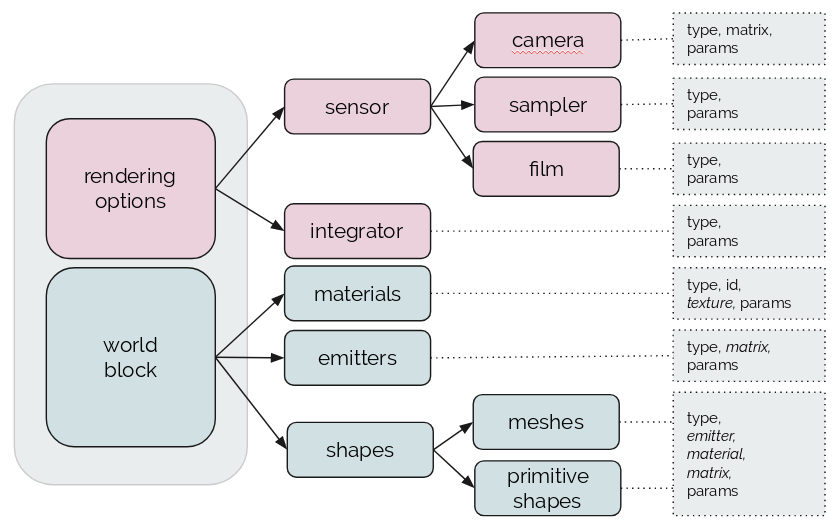
\includegraphics[width=0.6\linewidth]{figs/3_system_architecture/canonicalrep.png}
\caption{Illustration of the canonical scene representation.}
\label{fig:canonicalrep}
\end{figure}

\subsubsection{Scene-wide Rendering Options}
A set of directives specifying the integration and sampling techniques used for
rendering, camera and film properties. These directives are represented in a
structure with two fields: \red{a type and a list of parameters [EXAMPLE?]}.

\subsubsection{World Block}
A set of directives describing the shapes, materials and global emitters present
in the scene.

The \textbf{material} directive is represented in a structure with: a type \red{(examples of types?)}, an
id, an optional texture and a list of parameters.

The \textbf{shape} directive is represented in a structure with: a type (cube,
sphere, ...), an optional area emitter, an optional material reference, an
optional transformation matrix and a list of parameters.

The \textbf{texture} directive is represented in a structure with: a type, an id and a list of parameters. \red{[Where are the textures themselves stored?]}

The \textbf{global emitter} directive is represented in a structure with: a
type, an optional transformation matrix and a list of parameters.

\subsection{The Export Module}
After the data is loaded into our canonical
representation, it can be converted into any of the supported formats.

When converting scene representations, there are several delicate cases to
consider. The matrix transformations, the native shape
directives, the environment mapping coordinates and, mostly, the materials are
some of the directives that vary greatly between renderers. 

% \subsubsection{Converting Matrices}
\textit{1. Converting Matrices} \\
There are several issues to consider when converting matrices between renderers.
A few things we had to keep in mind were: does this renderer use a left or right
coordinate system? Does this renderer represent matrices in the scene file using
the inverse-transpose? How is the object-world transformation represented for
shapes?

Mitsuba uses a right-hand coordinate system, while PBRT and LuxRender use a
left-hand one. This meant that, when converting between Mitsuba and the other
two, we had to mirror the x-axis of all camera matrix transformations. This was
also the case for environment mapping positioning and object-world
transformations.

\green{Furthermore, Mitsuba scene files have their camera position specified as a 
world-to-camera transformation matrix, while PBRT and LuxRender scene files have 
theirs as a camera-to-world transformation matrix. Therefore, converting the 
camera positioning between Mitsuba and the other two renderers means we have to 
compute the inverse transpose of this transformation matrix.}

% \red{Mitsuba also has its camera transformation matrix specified as a camera-to-world
%  transformation, while PBRT and LuxRender do not. Therefore, when converting the
% camera look-at matrix between these renderers, we had to compute the inverse
% transpose of the specified matrix. }

% \subsubsection{Converting Materials}
\textit{2. Converting Materials} \\
Materials are maybe the most delicate aspect of scene conversion. Materials have
spectral and roughness properties that absolutely must be gotten right when
converting scenes. However, most renderers have very different implementations
for common subsurface scattering models (called BSDFs), making it hard to
predict the relation between their parameters.

Mitsuba uses a more physics-oriented approach: a material can be diffuse,
conductor, dielectric, plastic, translucent, or a bumpmap.
There are other types of materials, but those were not contemplated in our PoC.
The material type in Mitsuba changes should the material contain any form of
surface roughness, becoming a ``rough'' version of itself (for instance, a rough
metal becomes a roughconductor).

PBRT and LuxRender materials have roughness parameters, making it unecessary to
change the material's name.

The major problem was faced when converting metals from and to LuxRender. PBRT 
and Mitsuba use the index of refraction ($\eta$) and the absorption 
coefficient (\textit{k}) in each channel in order to compute material's 
reflectance. LuxRender, however, uses a Fresnel texture, which can specify a 
single value of $\eta$ and \textit{k} for all channels, or specify an RGB 
color. Therefore, getting a converted metal color between LuxRender and the 
others is very difficult, and was not implemented for this PoC. \\

\textit{3. Converting Shapes} \\
Shape directives can be split into two categories: primitive shapes, which can
be used to specify simple geometry such as cubes, rectangles, spheres and disks;
and 3D meshes in external files.

Converting meshes between renderers is simple, as all of them have directives
for this exact purpose. However, PBRT does not support Object File Wavefront 3D
(.obj) files - these must be converted by the user with mesh converting tools.
Our system issues a warning, making the user aware of this problem.

\green{Primitive shapes are a bit more complex. Mitsuba has directives for both cubes 
and rectangles, while PBRT and LuxRender do not. Mitsuba's cube and rectangle 
primitives define, respectively, 8 and 4 unitary points which can be modified by 
a transformation matrix. In order to reproduce these directives in PBRT and 
LuxRender, an inbuilt triangle mesh directive must be used, specifying each 
point that will compose the shape, which points form a triangle, each point's 
normal and the uv coordinates for this mesh.}

\green{The reverse process - converting PBRT and LuxRender triangle meshes into 
primitive Mitsuba shape directives - is more complicated. Since Mitsuba's 
primitive cube and rectangle directives have predefined coordinates for each 
vertex, to convert the points specified in the PBRT/LuxRender directive into 
these coordinates means finding the transformation matrix that transforms one 
into the other. }

% Since the triangle mesh directive specifies each points in world coordinates, 
% The reverse process, however, is more complicated. The triangle mesh directive
% specifies the coordinates, normal and uv mapping for the points forming a
% triangle. In order to recover a transformation matrix for the corresponding
% Mitsuba primitive, \red{these points have to be multiplied by the original Mitsuba
% canonical coordinates in the correct order.}

\textit{4. Converting Global Emitters} \\
Global emitters can used to emulate environment lighting, such as the sun, the
sky or even environment mapping. Converting these emitters can be tricky, mainly
because renderers don't implement the same algorithms and directives. For
instance, Mitsuba and LuxRender implement sun and sky algorithms; PBRT doesn't.
However, these directives can be converted from Mitsuba and LuxRender to PBRT. A
sun directive can be simulated in PBRT with a distant light. A sky directive can
be simulated using an environment mapping of a clear sky.

The inverse conversion can be a bit tricky. Converting a PBRT distant light into
a sun directive is a very straightforward conversion. Converting a PBRT
environment mapping into a sky directive is not: how could the converter know
whether the environment mapping is in fact an adaptation of a sky light? We
solved this issue by interacting with the user whenever an environment map
directive is found - we ask the user whether (s)he would like to use a sky
emitter or not.

Another sensitive point to consider is converting environment mapping 
indexation. In PBRT and LuxRender, environment maps' uv coordinates are indexed 
using spherical coordinates (\textit{theta} and \textit{phi}). Meanwhile, 
Mitsuba uses Cartesian coordinates (\textit{x}, \textit{y} and \textit{z}), as 
shown in Figure \ref{fig:mitdocemitter}. 

\begin{figure}[h]
\centering
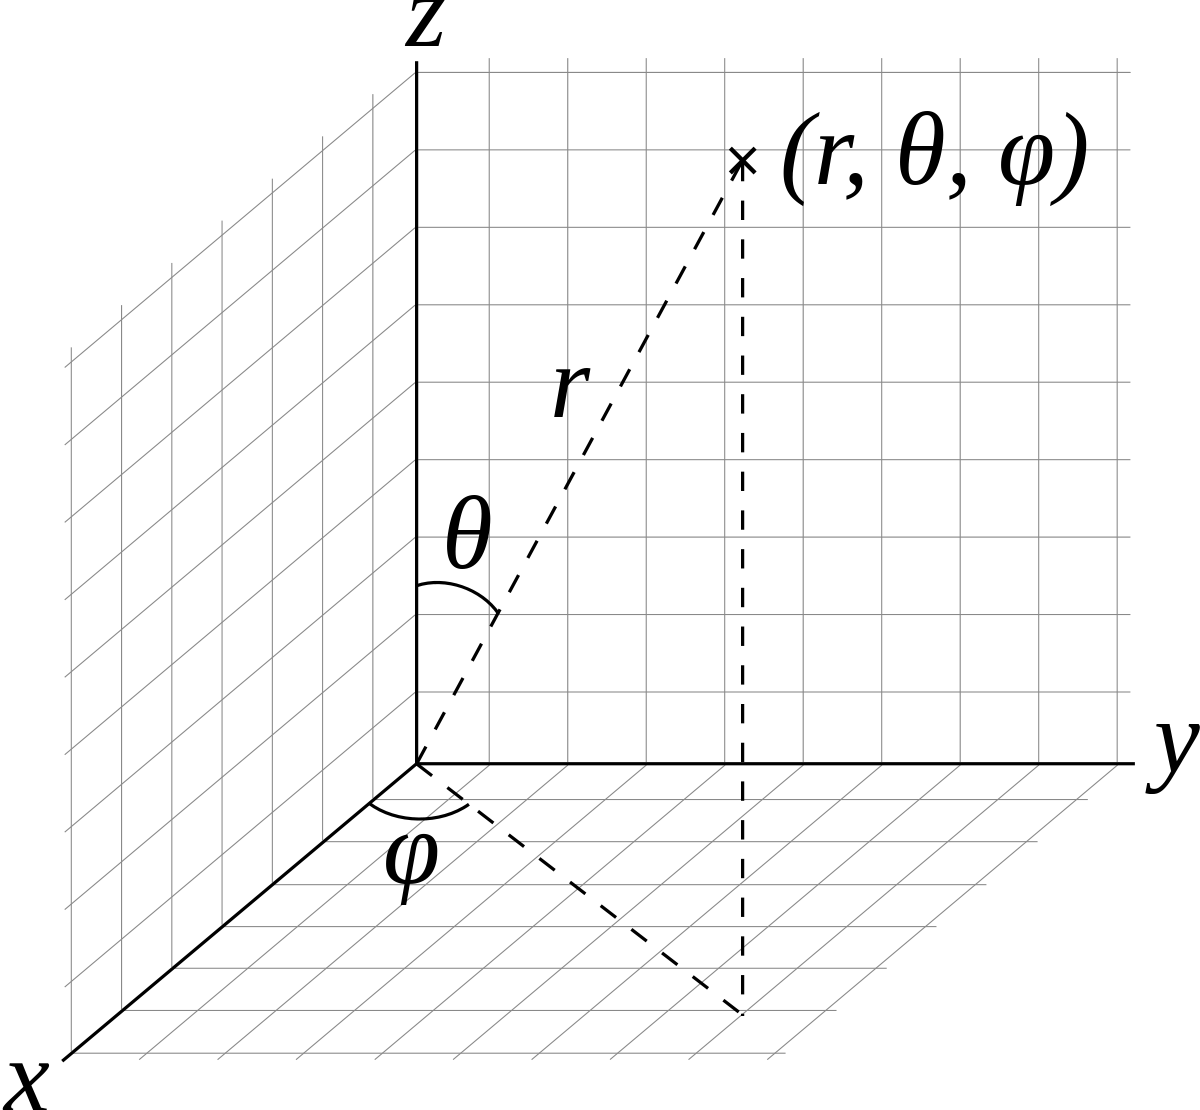
\includegraphics[width=1.2in]{figs/3_system_architecture/spherical_coordinates.png}
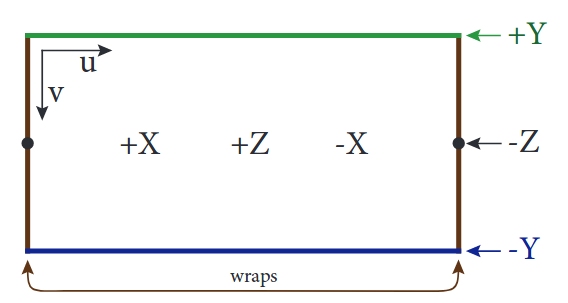
\includegraphics[width=2.0in]{figs/3_system_architecture/mitdocemitter.png}
\caption{Illustration of the coordinate conventions used by PBRT and LuxRender 
(left) and by Mitsuba (right) for indexing environment map uv coordinates.}
\label{fig:mitdocemitter}
\end{figure}

This conversion can be done by applying a transformation matrix on the 
environment map, rotating the \textit{x}, \textit{y} and \textit{z} axes to match the diferring axis setup. 
